\documentclass[12pt]{article}
\usepackage[utf8]{inputenc}
\usepackage{graphicx}
\usepackage{indentfirst}
\usepackage{hyperref}
\hypersetup{
    colorlinks,
    citecolor=black,
    filecolor=black,
    linkcolor=red,
    urlcolor=black,
}
\usepackage{caption}
\usepackage{subcaption}


\title{\textbf{The European Economic and Monetary Union} \\ \vspace{10 pt} \textit{What are the problems with the economic policy framework of the EU and the eurozone ? How can they be fixed ?}}
\author{Cheniour Maxime \\ Cinquanta Octave}
\date{January 2020}

\begin{document}

\maketitle

\tableofcontents

\section{Introduction}

The EU was created in 1992 following the Maastricht Treaty. It replaced the European Economic Community, whose aim was purely economic, to become a much larger institution which greater purposes. The EU is based on three pillars. The first one is the European Community, that includes single market, customs union,  economic and monetary, union common agricultural policy, and structural policy. The second one, the Common Foreign and Security Policy, gives a loose informal cooperation in foreign policy. The third and last pillar is the Cooperation in Justice and Home Affairs, which addresses the need for immigration services, interaction between the police, customs, and justice ministries of member states. The EU later triggered the birth of a eurozone, whose goal was to preserve the price stability within the union and strengthen it economically. \\
This work will be focused on the European Union’s policy framework, the eurozone and their various problems, as well as the potential responses to the latter.

\section{The Problems of the EU and the eurozone}

\subsection{The Stability and Growth Pact}

Firstly, we will take a look at different issues within the EU’s roots, namely its basic and defining rules. Let us take the case of the Stability and Growth Pact. This pact was established in 1997 when the EU’s member states decided to reinforce the monitoring of and the coordination of national fiscal and economic policies in order to implement the debt and deficit limits established by the Maastricht Treaty. This Pact is composed of two arms. The preventive arm aims to ensure correct budgetary policies over the medium term by giving the guidelines for member states' fiscal policies and planning during normal economic times, all the while taking into account the ups and downs of the economic cycle. This arm can initiate a Significant Deviation Procedure that gives a member state an opportunity to fix a divergence from their Medium-Term Objective or a path that leads to adjusting their MTO as to not trigger an Excessive Deficit Procedure. The corrective arm makes sure that member states adopt suitable policy responses to amend excessive deficits or debts by implementing the Excessive Deficit Procedure. The EDP is only launched under specific conditions when a member state has breached or is about to breach the deficit threshold of 3\% of its GDP, or when he has violated the debt rule, meaning having a debt of over 60\% of its GDP that is reduced slower than 1/20 of its total in a year, this being measured and averaged on 3 years. The countries in EDP are given a 6-months deadline to follow the recommendations on the path to correct their excessive deficit during a defined time frame. If a member state has been sanctioned under the Preventive arm already or his threshold breach is severe enough, he may face a sanction under the form of a 0.2\% of its GDP deposit without interests. Now that we’ve seen the Stability and Growth Pact in details, we can start looking at its flaws. First of all, though it may not be obvious, but its threshold values are far from being flexible enough, and especially for many weak European countries. This has been shown in 2017 when seven eurozone member states were sent a warning letter by the European Commission because of a potential deviation from the budgetary norms that were prescribed this year. These members were Portugal, Cyprus, Lithuania, Finland, Spain, Belgium and Italy. The requirements of this pact actually prevent a number of member states to implement a policy for economic growth, and this does not only concern the weakest countries of the Union. This can be seen with the fact that even countries like Belgium, one of the countries who established the EU, and Finland, a country with a usually rather strong economy, are seen as deviants from the norms of the SGP. The presence of those countries on the warning list only deepens the doubts one can have concerning the set rules of the eurozone and in particular this pact. Due to their weak growth, some member states are forced to spend more in order to stimulate the consumption and production of their economy, which then usually makes them breach the 3\% threshold set by the SGP. There is also that the European Council in Brussels is failing to accelerate the harmonization of the economical framework, which could be done by spreading equally the financial burdens among different social groups, as well as setting the same flat-rate system among all member states. All the while the Council struggles with tackling expansive tax evasion and regulating fiscal paradises. It is also important to remember that deviating from the SGP is also possible the other way around. The EU rules concerning the maximum level of trading surplus is set to 6\% maximum per year. Germany has been increasing its exports towards the other member states of the eurozone since 2011, and has been breaching the rules for a while. In 2015 its trade surplus was of 8.8\%. But regarding the case of Germany breaching the SGP, the Council does not apply the same treatment as for Italy’s case, who has been forced the adopt a lot of measures in order to fix its budgetary deficit. This decision shows the EU rules as being very asymmetric and contributes to a lack of cohesion between different member states. We can take a look at the following graph for the MTOs of the EU these past years. (Figure \ref{Figure 1})

\begin{figure}
    \centering
    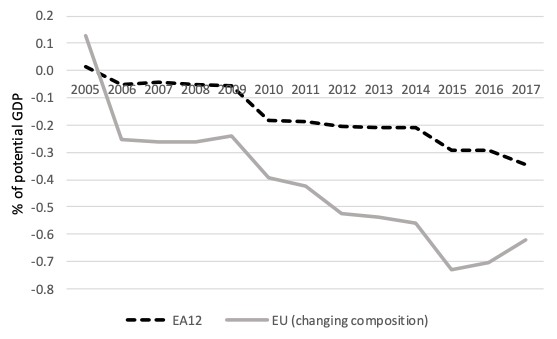
\includegraphics{fig2.png}
    \caption{Evolution of the average MTO}
    \label{Figure 1}
\end{figure}

On this graph, the black dotted line represents the evolution of the average MTO for the EA12 (which means Austria, Belgium, Finland, France, Germany, Greece, Ireland, Italy, Luxembourg, Netherlands, Portugal and Spain) and the grey line shows this evolution for the complete EU, so it includes the countries that were part of the EU at the time of each year’s data. We can see a rise of debt levels and that the objectives themselves are becoming less and less ambitious. This graph allows us to affirm the apparent weakness of the SGP’s preventive arm. Since we have talked about the first arm, we will now see the second and thus look at another graph. (Figure \ref{Figure 2})

\begin{figure}[ht]
    \centering
    
\includegraphics{fig1.png}
    \caption{Evolution of the percentage of potential GPD required}
    \label{Figure 2}
\end{figure}

On this graph, the black boxes represent the total percentage of potential GDP required for fiscal adjustment per year. We see that there is a major peak during the years of the European sovereign debt crisis, as it reaches almost 1\% in 2012. We can also use a data analysis made by Jasper De Jong and Niels Gilbert using data taken from the European Commission's forecasts. They aim to create real-time fiscal reaction functions for some member states between 1999 and 2017. Their results allow us to obtain that the EDP is significantly affecting the actual and planned fiscal policy. An EDP larger than 1\% of GDP makes of forecast of almost 1\% and an actual consolidation of 0.8\%. This shows that the EDP shapes in a significant way the fiscal policy, and it especially did during the after years of the crisis. \\
\\
We have seen the Stability and Growth Pact and its numerous flaws, mainly the facts that his preventive arm is too weak and that its corrective arm is in fact effective but too procyclical.

\subsection{The EU economic model, old and inefficient}

After discussing a problem lying at the origin of the EU's policy, we will now see why its economic model has aged badly, as it did no evolve enough and is now considered late. Indeed, Europe possesses a number of internationally renowned companies, but all of them are more than 20 years old. There is no such equivalent as today's Google, Amazon or Facebook in Europe. And concerning the new technologies of this century, what some call the 'fourth Industrial Revolution', Europe is far from involved. This uninvolvement is revealed also when looking at certain events earlier this year, specifically the tariff war between the USA and China. In terms of machine learning, China has a rather impressive development and owns companies that could threaten the ones located in the Silicon Valley. This is why in this 'war', China was the target chosen by Donald Trump. 30 years ago, when the different euro policies were being planned, it was thought that this single currency would improve the market's efficiency and engender a better and faster economical growth. However, the actual situation is rather far from it, and the performances of the member states of the eurozone isn't doing any better if not poorer. Recent health checks on the eurozone show that its growth is still chronically weak. Some countries are seen to have taken a toll recently, as Italy has known five recessions in the span of 20 years, and Germany barely escaped it towards the end of 2018 and the beginning of this year. The global slowdown of the economy has perturbed their export-focused economy harshly. The eurozone in general has known a small growth of 0.2\% during 2019's second and third quarters. (Figure \ref{Figure 3})

This graph shows the evolution of the GDP growth rates in percentage throughout the years 2007 to 2019, each year divided in four quarters. The data stops at the second quarter of 2019 here, however the third quarter has a growth rate of 0.2\%, just like the second one, and the data for the fourth quarter is yet to be issued. This graph presents two curves, one for EA19 (this includes the countries from the EA12, as well as Slovenia, Cyprus, Malta, Slovakia, Estonia, Latvia and Lithuania) and another one for EA28 (meaning the complete EU), and both stand for their respective GDP growth rates. The growth rates are mostly stationed between 0 and 1\%, although they become negative twice : once between 2008Q1 and 2009Q2 corresponding to the global financial crisis and the second time from 2011Q3 to 2013Q2 corresponding to the sovereign debt crisis. Overall, the GDP growth rates are rather low, usually around 0.5\%, and recent years have been mainly really low growth. The presence of two curves on this graph allows us to compare the growth rates of the eurozone (EA19) and of the EU (EA28). We can see that mostly everywhere the rates are higher for the EU, furthermore highlighting the existence of flaws in the eurozone.

\begin{figure}
    \centering
    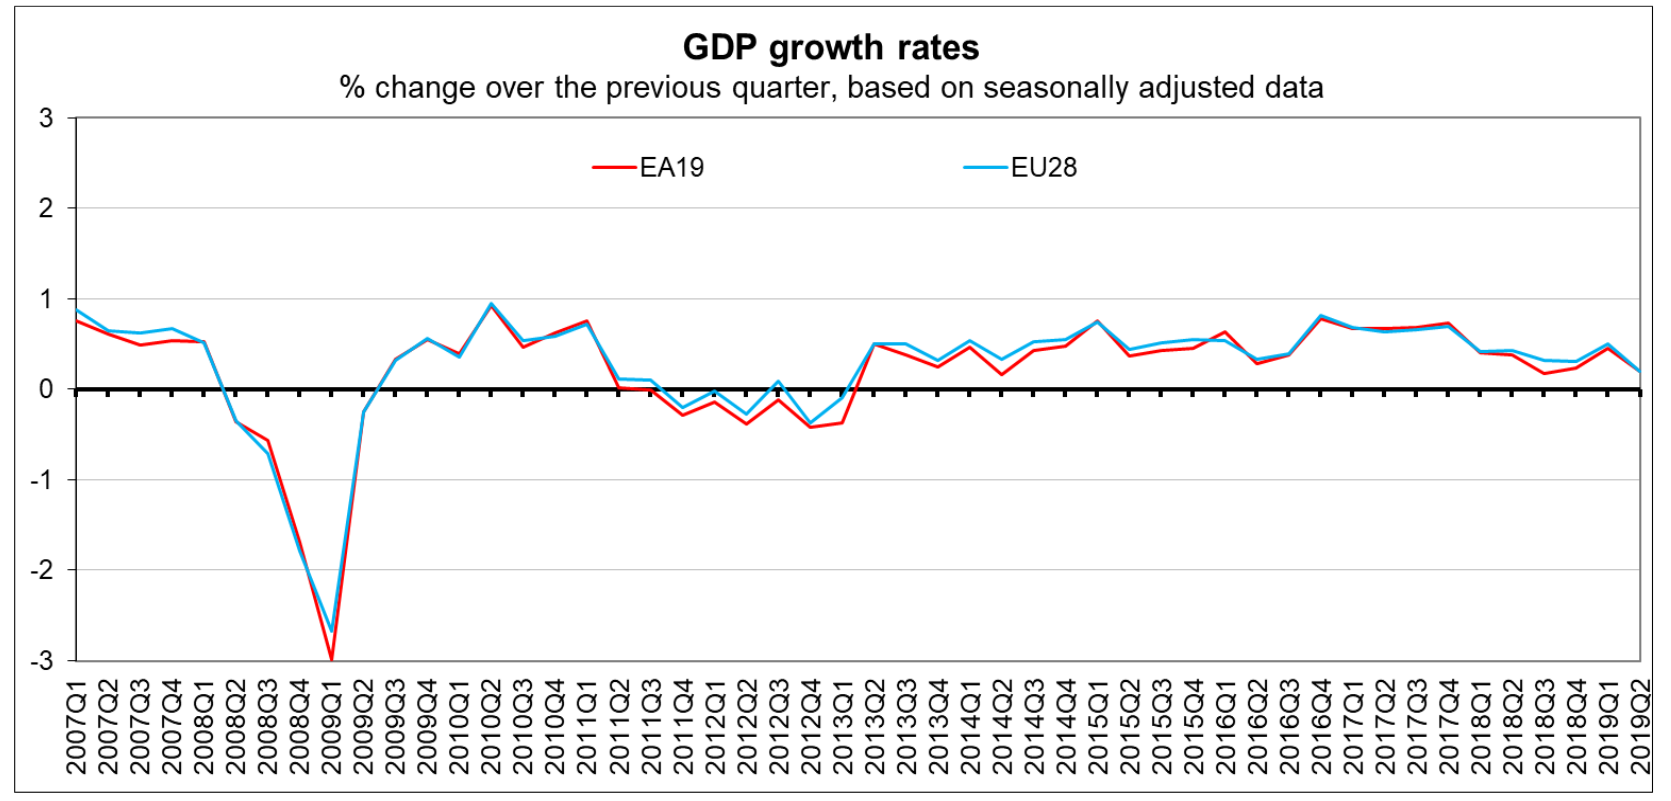
\includegraphics[width=135mm,scale=0.5]{fig3.png}
    \caption{GDP Growth Rates of the eurozone}
    \label{Figure 3}
\end{figure}


This growth rate has been lifted for a short period of time thanks to a number of stimuli from the European Central Bank. The beneficial zero interest rates and Quantitative Easing (when a state buys securities from the market to increase the money supply) are no longer having an effect. In order to correct Europe's failing growth, it is necessary to first fix the various problems in the base policy of the EU. During the crisis of 2008, the absence of a political foundation for the euro impacted the economy. When the crisis emerged, the USA and the UK were able to rapidly cut the interest rates and switch to unconventional monetary policies like the QE, but the eurozone took too much time doing so. It seems to be due to the conservative nature of the ECB, as well as the lack of any kind of mechanism created for this effect. This slowness had two major consequences : the return to growth for the eurozone took muck longer and banks were now filled with many non-performing loans. The USA were able to socialise their major debts in order to be able to lend again. This left the European banks left vulnerable in case of another crisis. In any case, Italy today is becoming more desperate to revive its own economy, and would use any means. And at the beginning of this year, its government announced their participation in the Chinese Belt and Road initiative, a project consisting of building ports, railroads, bridges to link Africa, Europe, the Middle East and Asia. These news show the weakened status of Europe. Our president Macron firmly believes the solution to these problems is closer integration. He wishes for the existence of a minister unique to the eurozone and dedicated to managing taxes and fiscal policies for the zone. However for this idea to come in the light is necessary the support of Germany. Angela Merkel isn't willing to cooperate because Germany has been doing better in the Union and its government would be expected to spend money in poor countries of the eurozone. This plan is in fact a good idea, as it would fill in the missing political half of the eurozone, and that another solution considered is leaving the eurozone. \\
\\
We have now seen why the European economic model is considered old and inefficient, as well as a major flaw which is the lack of a political structure for the eurozone. 

\subsection{The asymmetric behaviour of the members}

Before the implementation of the euro, many feared the appearance of asymmetric shocks on a region possessing little inter-country labour mobility and no fiscal policy in common. Researches had shown that Europe's periphery had been hit by major idiosyncratic shocks. Many felt this would create some difficulties for the single currency. Yet looking at the last 10 years and today's issues, the effects of asymmetric shocks aren't what strikes the eye. Even the biggest shock, called the Great Recession, is very symmetric. The cause of asymmetric declines of GDP is in fact due to the different behaviour of the members' economies. A difference in behaviour between countries with different economies and political structures was to be expected but not to the point where many of their actions would threaten the single currency. The most evident differences are seen between the North (Germany, Austria, the Benelux and Finland) and the South (Portugal, Spain, Italy and Greece). The first example to look at is in the realm of fiscal policy. The North quickly took in fiscal austerity, unit cost control and a growth strategy oriented on exports. The same could not be said for the South. This can be seen looking at the steep decline in long-term interest rates, allowing for a smooth reduction of government debt. It is particularly evident when comparing the Belgium and Italy cases. (Figure \ref{Figure 4}) In 1999, public-debt ratio were of 121\% of GDP in Belgium and 128\% in Italy. In 2008, they had been reduced to respectively 91\% and 113\%, much more in Belgium, even though the long-term debts had fallen much faster in Italy. During this period, in Greece and Portugal debt actually rose, and in Spain low interest rates allowed a huge housing bubble and increased private debt. We can study another important divergence, this time looking at the very different growth rate and productivity between the North and the South. At the time of Bretton Woods, inflation was similar for the North and South, but the last 12 years are the complete opposite of this. (Figure \ref{Figure 5}) The wage inflation in Spain and Italy was higher than in Germany, the productivity growth was dim in the South and strong in the North. Commission estimates are suggesting that the intra-eurozone exchange rate in the South was appreciated by as much as 25\% of the one in the North. The fate of this zone remains lower growth once again, or to be forced into nominal devaluation. Both those ends can be avoided with a proper fiscal union, but at a certain cost. And it is really unlikely that the North would accept a fully-fledged fiscal union. There are multiple reasons for this assumption, and more than a simple question of money. This is mainly a question of trust, and this is shown by the rigid conditions put on Greek politicians, and also by Eurobarometer on how much trust citizens of a country have in citizens of their neighbouring countries. We see that the divergences have in fact grown since the implementation of the euro. What was expected was for known gaps in the governance to diminish, when in reality they widened instead. We can use a few examples. (Figure \ref{Figure 6}) There are the perceptions of corruption and the regulatory quality, that both worsened in the South for the last 10 years. Also the importance of the underground economy that has gotten a bit smaller in the South, but also in the North so the huge gap still remains. The presence of the rule of law has also lowered in the South, a fact that is quite worrying.

\begin{figure}
    \centering
    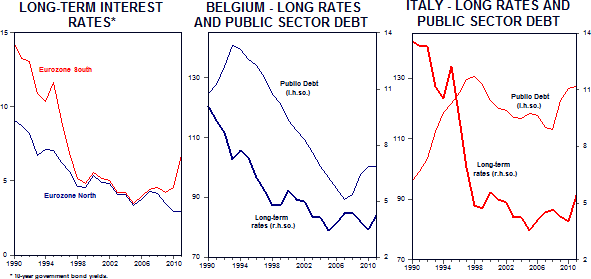
\includegraphics[scale=0.5]{fig4.png}
    \caption{Long-term interest rates and public-sector debt}
    \label{Figure 4}
\end{figure}

\begin{figure}
    \centering
    \begin{subfigure}{0.5\textwidth}
    \centering
    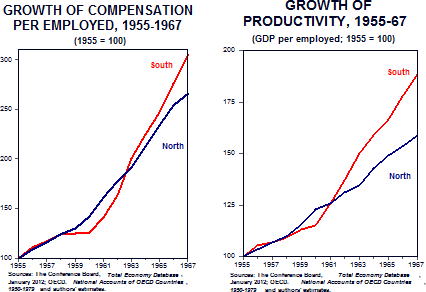
\includegraphics[width=0.9\linewidth]{fig5.png}
    \caption{Bretton Woods}
    \end{subfigure}%
    \begin{subfigure}{0.5\textwidth}
    \centering
    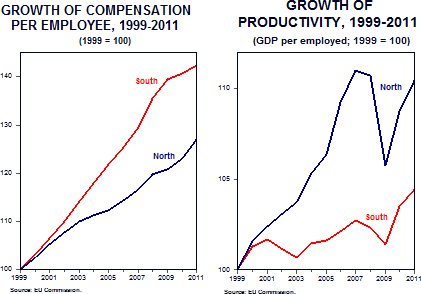
\includegraphics[width=0.9\linewidth]{fig6.png}
    \caption{Eurozone}
    \end{subfigure}
    \caption{Wage and Productivity Growth}
    \label{Figure 5}
\end{figure}

\begin{figure}
    \centering
    \begin{subfigure}{0.5\textwidth}
    \centering
    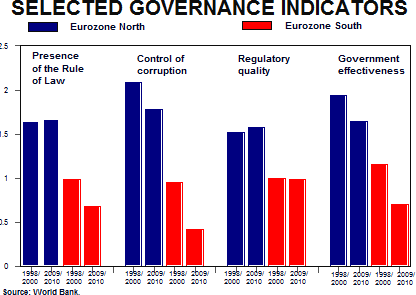
\includegraphics[width=0.9\linewidth]{fig7.png}
    \caption{The Indicators}
    \end{subfigure}%
    \begin{subfigure}{0.5\textwidth}
    \centering
    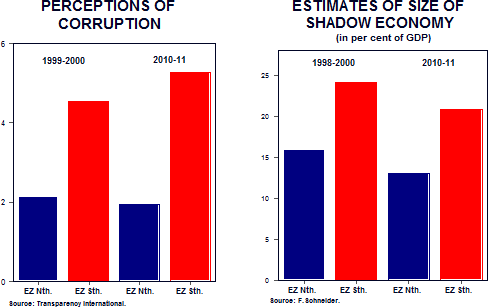
\includegraphics[width=0.9\linewidth]{fig8.png}
    \caption{Corruption and Shadow Economy}
    \end{subfigure}
    \caption{Governance Indices}
    \label{Figure 6}
\end{figure}



So now we saw the different problems linked to the asymmetric behaviour of the members and what causes them.

In the end we were able to analyse the EU and the eurozone, and found multiple types of problems within them : some come from the very set rules of the union, like the Stability and Growth Pact, some are caused by the fact that the economic model of the EU has aged and became inefficient and that there is a lack of political structure, and some also come from the different behaviour of some members of the union.

\section{Possible Solutions for the eurozone}

Now, the eurozone has its own share of problems as previously stated, but we cannot really say that it had a bad influence on Europe. Quite the opposite as, being a unique money shared between 19 countries, it has made trade between European countries a lot easier for most people, as they no longer needed to look at exchange rate, currency risk hedges or monetary policy decisions from different governments, among many issues.
The euro is an international money which is stable, has a low inflation and is recognized worldwide giving stability and confidence to some citizens who didn’t experience this since decades. Since its inception, eurozone GDP per capita has increased by 52\% going from around 21 000 euro to 32000 euro and the participation rate is higher in the eurozone than in the United States. Nonetheless inflation has reached an average of 1.7\%, a rate lower than the ones recorded in the three decades preceding the inception of the eurozone.  
Now are there solutions to the problems plaguing the euro zone or will we need to get rid of this currency ?

\subsection{Erasing Public Debts ?}

Erasing public debts has its own issues and dangers. The government may conduct themselves in an opportunistic way, meaning doing nothing to keep the public finances afloat. Thus, it is unadvisable to fully erase the debts. What would be favorable is a restructuration, step by step. It is possible to partially erase the public debts of the countries having the most difficulties, but it is better to be careful as, the more we erase, the higher the future loans will be. Moreover, it will be necessary to replenish the banks, as they possess the sovereign bonds. To reach term, the banking union project is vital as, the main problems are the debts in the private sectors, mainly in finance, households and compagnies, and the intrinsic relationship between the government and the banks.
Before the 2008-2009 financial crisis public debt diminish slowly but surely, omitting certain countries. But following the event, public debts grew due to the bailout of the banking sector, the fall of tax revenue during the recession and, during the sovereign debt crisis the increase in the interest charges. Concerning the private sector, we can see a steady rise of the debts, primarily with the housing. This can be observed mostly in Greece, Spain, Ireland, Italy, Portugal and Finland.
Now a days, the private sector tries to deleverage. We can see that the debts of the Irish and Spanish households have lowered since 2009. But, to reduce a debt, the private sector is selling assets. It follows that the assets price reduces, which leads to other agents in financial difficulties, forcing them to also reduce their own debt. This could create a deflationary cycle. To counter this issue, we need buyers: those could be European Central Bank, the government or another country/company. In the first case the ECB has a monetary operation program. In the second case, an increase in public debt will be observed. And in the third case, either the country’s wealth will diminish or its debt will increase. Thus, it is not desirable that the government try to reduce the public debt too fast, as it risks leading us in a deflationary situation, especially as the restrictive fiscal policies do not allow to exit the recession nor to reduce the public deficit.
The close relationship between the government and the banks can be constraining in case of excessive debt of either of the two. If the government is a lender as a last resort to the banking sector and that the banking sector has a weak finance, then the government suffers increased interest rate. This can make it difficult for the government to reimburse and this can damage the bank’s assets, as they are the ones possessing the public securities. To conclude, growth support policies to ease the deleveraging of the private sector, and by that, from the public sector.

\subsection{Fiscal Federalism ?}

The fiscal federalism is a type of centralized public finance organization which takes count of the political tax, the public spending and debt management. In our context, two possibilities are considered: in the short term, it is about putting together the public debts and create Eurobonds to ease the access to the financial markets for the developing countries. In the long term, we want to implement a federal budget to cushion the impact on specific economies.

\subsubsection{Debt Pooling}

Pooling debt means giving euro area Member States the possibility to borrow by issuing bonds (denominated in euros) without bearing a specific default risk premium, because these bonds are securities on which the identity and quality of the issuer does not correspond to the borrowing State, but to an entity common to the countries, namely the euro area as a whole. In other words, it is the euro area that is the issuer of these bonds, which are therefore called Eurobonds. For the most heavily indebted states, which are subject to a higher default risk premium than other countries, this solution allows for lower interest rates on government bonds. But for the least indebted States, this implies a rise in interest rates if the euro zone entity is rated lower than them by the rating agencies. This is possible if we consider that this entity includes countries whose public debt is very high as a proportion of GDP (or the net assets of some countries are not sufficient to offset the liabilities of others). Unsurprisingly, when a Eurobond project in 2011 was discussed, Italy was a strong supporter, while countries with AAA-rated public debt were reluctant (such as the Netherlands, Finland, and Germany). The major disadvantage of this type of project is that it presents a moral hazard. If states do not bear the responsibility for an increase in their indebtedness through a higher risk premium and therefore higher interest rates on their loans, then there is no incentive to reduce public deficits and public debts. However, in a monetary union, fiscal discipline is necessary to prevent major economic imbalances from endangering the monetary edifice. The Greek crisis unfortunately illustrates this need. When we share a common currency, we must agree to play by its rules. And if these rules of the game are considered irrelevant, then one must negotiate an amendment to the texts or leave the union (or not enter the union for those who do not already participate). To limit the moral hazard of Eurobonds, a proposal to create "blue bonds" had already been made in 2010 by French economist Jacques Delpla and German economist Jakob von Weizsäcker. Their proposal consists of pooling part of the public debt: each country would be authorized to issue blue bonds, for an amount not exceeding 60\% of its GDP (this is the public debt criterion of the European texts). These blue bonds correspond to Eurobonds. They would be issued at low interest rates, because the entire euro zone guarantees repayment.
 Any country, which would need to borrow more than 60\% of its GDP, would have to issue its own bonds ("red bonds") and, consequently, would have to bear higher interest rates (specific risk premium, as the debt is not guaranteed by the other partner countries). Within this framework, there would be an incentive to avoid public debt exceeding too much 60\% of GDP. This is an interesting proposal, but it suffers from an important theoretical limitation: the 60\% threshold is arbitrary. It is unfounded. It is not a limit beyond which the debt is unsustainable. French economists from the Conseil d'Analyse Economique (CAE) have recently drawn up a project to "complete the euro", in which the idea of Eurobonds is also included. A European Debt Agency (EDA) would buy back national sovereign bonds and issue Eurobonds in exchange. This debt exchange would represent 20\% of the GDP of the country concerned, and would not be a debt buyback, since the country concerned would have to repay the debt assumed by the EDA. The interest of the proposal is to establish repayment conditions that aim to protect the most indebted countries against the vagaries of the financial markets: they would have to repay after 10 years over a period of 15 years (at interest rates lower than those of the market).

\subsubsection{A Federal Budget}

The budget of any state, federation or monetary union generally has three functions (according to Richard Musgrave's classification): a resource allocation function (provision of collective goods and services, sectoral policies), a stabilization function for the economy (cushioning the effects of shocks), and an income redistribution function (reducing income inequalities). A federal budget for the euro area appears necessary for stabilization, because increasing integration (free mobility of goods, workers, financial capital and enterprises, common budgetary rules) limits the ability of Member States to pursue stabilization policies. The European Union has a budget that is not suited to a stabilization objective, as the size of this budget is very small (1% of the national income of the 28-member countries) and its structure is based, for the most part, on spending on allocations for agriculture and redistribution in favor of regions whose development is lagging behind. As for the euro zone, it is a monetary union that does not have its own budget. This is an unprecedented specificity, because a monetary union is generally associated with a budgetary union, which requires a political union. In other words, in order for the euro zone to have a federal budget, we must also think about setting up a government that executes this budget and a Parliament that authorizes it. In order to make things less complicated, it might be conceivable that part of the EU budget could be devoted to the eurozone's stabilization needs.
How does a federal budget work in terms of stabilization? Jeffrey Sachs and Xavier Sala-I-Martin showed, in the case of the United States, that when a state's per capita income falls by 1 dollar, the taxes it pays to the federal government fall by about 34 cents, while the transfers it receives from the federal government increase by about 6 cents. Net changes in federal payments and transfers thus offset 40\% of a 1 dollar drop in regional income. The degree of stabilization is therefore 40\%.  It varies from one study to another, between 15 and 30\% depending on the methodology used, the countries considered (United States, Canada, Switzerland, Germany) and the period covered. However, the stabilization function is difficult to separate from the redistribution function. In principle, at the level of a federation, stabilization aims at ensuring that any state, region or province, rich or poor, benefits from automatic transfers or tax reductions as soon as it suffers a temporary reduction in income due to specific unfavorable disturbances. Redistribution, on the other hand, consists of transfers to the least developed states, regions or provinces, whether or not they are facing shocks. In this respect, if we want to set up a federal budget for the euro area, then we have to think about the level of stabilization: are we aiming at a stabilization of the income of states (regions) or of individuals? Moreover, federal transfers are likely to disrupt another mechanism for adjusting to shocks, namely labor mobility (one of the criteria for an optimal currency area put forward by Robert Mundell in 1961). In the early 1990s, Canadian economist Thomas Courchene explained what has come to be known as “the Canadian disease”: the unemployment insurance system, which was part of the federal system of inter-regional (inter-provincial) transfers, may have induced rent-seeking behavior in the form of migration flows to regions of high unemployment, because the number of weeks worked required to benefit from the transfers depended on the regional unemployment rate: 20 weeks for low unemployment areas, but 10 weeks for high unemployment areas.
The establishment of a European federal budget faces political obstacles, because it implies a loss of sovereignty in the tax field: Member States must accept that a supranational authority levies a tax on their citizens or shares with them part of the national tax revenues, and that it decides on the allocation of its tax revenues (on the basis of pre-defined rules). In practice, there are three possibilities for setting up this type of budget: creating a European tax, centralizing part of the tax revenue or organizing cyclical transfers.
Firstly, European taxation should have a broad and, if possible, stable (predictable) tax base, and it should hit the most mobile tax bases (such as companies, which are most likely to make tax optimization by taking advantage of national differences in regulation). Corporate income tax more or less meets these conditions (except for stability), but Member States are unlikely to agree to abandon this type of tax (and double taxation at national and EU level is not desirable). Indeed, in the medium term, they have constraints on reducing public deficits, and this type of tax has a significant (albeit diminishing) return. Given that a tax on financial transactions (bonds, shares, currencies, derivatives) is not effective at the national level, because the volume of transactions is decreasing (they are made elsewhere), it would be interesting to create such a tax at the European level. Luxembourg would have to be convinced to accept it (tax issues are voted unanimously in the EU). As its economy is highly specialized in financial services, Luxembourg fears that transactions would take place outside the EU if such a tax were created.
Secondly, part of the national tax revenue, collected on a given tax, could be shared with the EU (or the euro area). On this subject, let us return to corporate income tax: the definition of the tax base in the different countries needs to be standardized. At present, this tax has a lower effective rate than the legal rate, due to the many exceptions that reduce its base or amount (allowances, deductions, exemptions, reduced rates, reductions or tax credits). These exceptions correspond to what are known as tax expenditures. For example, France is in the unenviable position of having one of the highest statutory tax rates on corporate profits in the EU, but a relatively low effective rate (ratio of its amount to its base). Thus, is it not the country that taxes profits relatively more. However, in their choice of location, companies observe the legal (official) rates and not the effective rates (which have to be calculated). Harmonizing the definition of the tax base would also hamper the tax optimization practices of companies, and thus cause some Member States to lose less tax revenue. Then, after agreeing on the characteristics of this base (and in particular tax expenditure), agreement must be reached on the amount of national tax revenues, which would be allocated to the European budget: for example, each State's share could be equivalent to the share of domestic corporate profits in the GDP of the euro zone or in the total profits of EU (or euro zone) companies.
Thirdly, a less ambitious form of fiscal federalism is to organize cyclical transfers: countries with GDP growth above its potential pay transfers to the centralized budget and those with growth below receive transfers. There is, of course, a problem with transfers to the budget when everyone is in recession! Moreover, potential output is not measured precisely (valuation differences depending on the methodology). Therefore, another possible system is a system of federal transfers based on regional unemployment rate differentials (avoiding the old Canadian problems mentioned earlier). Alexander Italianer and Jean-Pisani Ferry had studied such a system in a 1992 article: A Member State would receive a transfer, proportional to its GDP, if the annual increase in its unemployment rate is higher than the Community (EU) average. For example, each difference of one point from the EU average would result in an annual transfer of one point of GDP received. Relative changes in unemployment rates of more than two points would not be compensated for. It may be thought that manipulation of unemployment data or incentives not to fight unemployment should be avoided. Simulating the operation of this stabilization mechanism, the authors find that a one-point decrease in relative GDP, which translates into a 0.18-point increase in the relative unemployment rate, would result in a 0.18 per cent of GDP transfer, or an 18 per cent degree of shock stabilization. They calculated that the budgetary cost of this mechanism would average 0.23\% of Community GDP over the period studied (1984-1991), ranging from a minimum of 0.06\% in 1990 to a maximum of 0.36\% in 1984. A similar system is found in the proposals made in a recent ACE note.

\subsection{The break-up of the monetary union ?}

A priori, a disappearance of the euro is not desirable. In addition to the gains of a single currency (lower transaction costs, better allocation of resources between territories, lower interest rates), we must remember the historical and political reasons for the creation of monetary union. It was France, in particular, which brought the single currency project to a successful conclusion by convincing Germany, which was reluctant to abandon the Deutsche Mark, to accept the project. It even almost forced Germany's hand: it was a condition set by French President François Mitterrand to German Chancellor Helmut Kohl in return for German reunification. In economic terms, France no longer wanted to submit to the constraints of the European Monetary System (EMS), a system of adjustable fixed exchange rates. Since the liberalization of capital movements between the main countries of the European Community in July 1990, the countries participating in the EMS were obliged to conduct their monetary policies in a coordinated manner with the aim of maintaining the exchange rates of their fixed currencies. They were losing the autonomy of monetary policy (except Germany), because if they set key interest rates at different levels (from the German rates), then capital movements would occur and currency exchange rates would deviate from the official parities. 
The EMS confronted them with the famous triangle of incompatibility formulated in the 1960s by the American economist Robert Mundell: you cannot have fixed exchange rates, free capital movements and an autonomous national monetary policy at the same time. However, the renunciation of fixed exchange rates was not compatible with the project of creating a single currency, which required a transition period with stable exchange rates, nor with the single market. The return to capital controls was also not compatible with the Single Market program. It therefore remained to abandon the autonomy of monetary policy, accepting the idea that it should no longer be conducted in accordance with internal economic policy objectives, but with the objective of fixing the exchange rate. To free itself from this constraint, France believed that by participating in a monetary union with Germany, it could participate in monetary policy decisions within a common central bank and steer decisions according to internal objectives. However, Germany insisted that the statute of the ECB should be enshrined in the EU Treaty and ensure that it is an independent institution, which takes its decisions on the basis of a primary objective of price stability, in the general interest of the euro area, and not on the basis of specific national interests.
If the euro area were to break up today, due to a lack of understanding and solidarity among its members, and if member countries had their own national currencies again, then they would have to choose an exchange rate regime for their currencies, since they are convertible on the international currency markets. The above reasoning shows that they are unlikely to choose a return to the EMS. Moreover, any system of intermediate fixed exchange rates (devaluations or possible revaluations if necessary) is vulnerable to speculative attacks, and defending the exchange rate becomes costly (in terms of foreign currency reserves, interest rates are too high to deter speculation). It is therefore quite possible that each country will adopt floating as its exchange rate regime. However, a flexible exchange rate does not have the same implications for countries with external deficits (such as Greece, Portugal, France) or external surpluses (such as Germany, the Netherlands, Belgium or Austria among others).
For countries with external deficits, a real depreciation of the currency, i.e. a fall in the relative prices of domestic goods and services compared to the prices of foreign goods and services, is necessary. The advantage of floating is that the correction of external deficits can be based on exchange rate adjustment (i.e. a nominal depreciation of the currency) and not only on a fall in domestic prices and costs. Adjustments are therefore less painful. However, it should not be assumed that currency depreciation is a panacea. While it favors exports of goods and services to the rest of the world (albeit with delays, since the volumes traded do not react immediately to exchange rate changes), it also leads to higher prices for imports of goods and services (and quickly, since the exchange rate is a relative price). However, the integration of economies into international trade is such that firms now need to import raw materials or capital goods before producing goods (although this is less true for services). Consequently, a depreciation of the domestic currency tends to increase their production costs. In addition, small countries are usually forced to borrow in foreign currency to finance public or private sector debt because their domestic financial markets are too narrow (insufficient participants). For them, a depreciation of the domestic currency implies heavier repayments. And even if a country can issue government bonds denominated in its own currency, the fact remains that if its currency tends to depreciate in foreign exchange markets, then interest rates on the bonds it issues will be higher, because foreign lenders will demand an exchange rate risk premium. Moreover, for Italy, adopting the euro allowed it to benefit from much lower long-term interest rates because it no longer faced an exchange rate risk premium. And it is also well known that the threats of Greek politicians to leave the euro area (if the country was not bailed out by the others) were not credible, because the cost of exiting in the middle of the crisis would have been exorbitant (collapse of the drachma and much higher interest rates). For countries with external surpluses, floating translates into an appreciation of the domestic currency against other currencies. This does not necessarily imply a loss of competitiveness, as it depends on the evolution of domestic costs and prices, nor does it imply a loss of market share, as it depends on the quality of international specialization (for some goods or services, foreign customers are willing to pay a high price if the quality is high or if the good or service has no close substitutes).

In conclusion, the euro area crisis illustrates a lesson from the literature on optimal currency areas, namely that a monetary union is not sustainable if the participating countries do not share the same economic policy preferences. The Dutch, Austrians, Finns and Germans are committed to compliance with the rules in general, and to fiscal discipline (balancing public finances) in particular. They are irritated by having to bail out countries of the South that flout the rules (Greece) or that have not taken measures to avoid a worsening of the economy, financial or external imbalances (the other countries of the South). One mistake has been to enlarge the euro area too quickly to small countries, believing that economic developments in these countries would not affect the euro area as a whole. One of the criteria for an optimal currency area is strong trade interdependence (contribution by Ronald McKinnon in 1963). However, the share of intra-euro area trade in Greece's foreign trade is relatively limited. At the very least, this criterion should be checked in the future, if a country is a candidate for the euro area. Similarly, it would be necessary to ensure that the country shares the same ethics with regard to the respect of the rules of living together. In the light of these criteria, it would not be surprising if the countries of the North were to consider a monetary union among themselves, if the member states were unable to agree on mechanisms for preventing and resolving crises. In any case, the member states should no longer ignore the criteria of the theory of optimal currency zones, which included a federal budget (Peter Kenen's contribution in 1969). All things considered, a dissolution of the euro zone must be avoided if it is a threat to the construction of Europe, which has brought us peace on the continent.


\section{Bibliography}
\subsection{Articles / Websites}
\begin{itemize}
\item VOX,\textit{ The Mixed Success of the Stability and Growth Pact}, by Jasper De Yong and Niels Gilbert
\item European Commission, Stability and Growth Pact
\item The Guardian, \textit{The European Union has bigger problems to deal with than Brexit}, by Larry Elliott
\item VOX, \textit{The problems with the Eurozone}, by Andrea Boltho and Wendy Carlin
\end{itemize}

\subsection{Figures}
\begin{itemize}
\item Figures 1,2,4,5,6 --- VOX, Figure 3 --- This time it is different
\end{itemize}

\end{document}
